\documentclass[addpoints, 12pt]{exam}%, answers]
\usepackage[utf8]{inputenc}
\usepackage[T1]{fontenc}

\usepackage{lmodern}
\usepackage{arydshln}
\usepackage[margin=2cm]{geometry}

\usepackage{enumitem}

\usepackage{amsmath, amsthm, amsfonts, amssymb}
\usepackage{graphicx}
\usepackage{tikz}
\usetikzlibrary{arrows,calc,patterns}
\usepackage{pgfplots}
\pgfplotsset{compat=newest}
\usepackage{url}
\usepackage{multicol}
\usepackage{thmtools}
\usepackage{wrapfig}

\usepackage{caption}
\usepackage{subcaption}
\usepackage{pdfpages}

\usepackage{pifont}

% MATH commands
\newcommand{\bC}{\mathbb{C}}
\newcommand{\bR}{\mathbb{R}}
\newcommand{\bN}{\mathbb{N}}
\newcommand{\bZ}{\mathbb{Z}}
\newcommand{\bT}{\mathbb{T}}
\newcommand{\bD}{\mathbb{D}}

\newcommand{\cL}{\mathcal{L}}
\newcommand{\cM}{\mathcal{M}}
\newcommand{\cP}{\mathcal{P}}
\newcommand{\cH}{\mathcal{H}}
\newcommand{\cB}{\mathcal{B}}
\newcommand{\cK}{\mathcal{K}}
\newcommand{\cJ}{\mathcal{J}}
\newcommand{\cU}{\mathcal{U}}
\newcommand{\cO}{\mathcal{O}}
\newcommand{\cA}{\mathcal{A}}
\newcommand{\cC}{\mathcal{C}}
\newcommand{\cF}{\mathcal{F}}

\newcommand{\fK}{\mathfrak{K}}
\newcommand{\fM}{\mathfrak{M}}

\newcommand{\ga}{\left\langle}
\newcommand{\da}{\right\rangle}
\newcommand{\oa}{\left\lbrace}
\newcommand{\fa}{\right\rbrace}
\newcommand{\oc}{\left[}
\newcommand{\fc}{\right]}
\newcommand{\op}{\left(}
\newcommand{\fp}{\right)}

\newcommand{\ra}{\rightarrow}
\newcommand{\Ra}{\Rightarrow}

\renewcommand{\Re}{\mathrm{Re}\,}
\renewcommand{\Im}{\mathrm{Im}\,}
\newcommand{\Arg}{\mathrm{Arg}\,}
\newcommand{\Arctan}{\mathrm{Arctan}\,}
\newcommand{\sech}{\mathrm{sech}\,}
\newcommand{\csch}{\mathrm{csch}\,}
\newcommand{\Log}{\mathrm{Log}\,}
\newcommand{\cis}{\mathrm{cis}\,}

\newcommand{\ran}{\mathrm{ran}\,}
\newcommand{\bi}{\mathbf{i}}
\newcommand{\Sp}{\mathrm{span}\,}
\newcommand{\Inv}{\mathrm{Inv}\,}
\newcommand\smallO{
  \mathchoice
    {{\scriptstyle\mathcal{O}}}% \displaystyle
    {{\scriptstyle\mathcal{O}}}% \textstyle
    {{\scriptscriptstyle\mathcal{O}}}% \scriptstyle
    {\scalebox{.7}{$\scriptscriptstyle\mathcal{O}$}}%\scriptscriptstyle
  }
\newcommand{\HOL}{\mathrm{Hol}}
\newcommand{\cl}{\mathrm{clos}}
\newcommand{\ve}{\varepsilon}

\DeclareMathOperator{\dom}{dom}

%%%%%% Définitions Theorems and al.
%\declaretheoremstyle[preheadhook = {\vskip0.2cm}, mdframed = {linewidth = 2pt, backgroundcolor = yellow}]{myThmstyle}
%\declaretheoremstyle[preheadhook = {\vskip0.2cm}, postfoothook = {\vskip0.2cm}, mdframed = {linewidth = 1.5pt, backgroundcolor=green}]{myDefstyle}
%\declaretheoremstyle[bodyfont = \normalfont , spaceabove = 0.1cm , spacebelow = 0.25cm, qed = $\blacktriangle$]{myRemstyle}

%\declaretheorem[ style = myThmstyle, name=Th\'eor\`eme]{theorem}
%\declaretheorem[style =myThmstyle, name=Proposition]{proposition}
%\declaretheorem[style = myThmstyle, name = Corollaire]{corollary}
%\declaretheorem[style = myThmstyle, name = Lemme]{lemma}
%\declaretheorem[style = myThmstyle, name = Conjecture]{conjecture}

%\declaretheorem[style = myDefstyle, name = D\'efinition]{definition}

%\declaretheorem[style = myRemstyle, name = Remarque]{remark}
%\declaretheorem[style = myRemstyle, name = Remarques]{remarks}

\newtheorem{theorem}{Théorème}
\newtheorem{corollary}{Corollaire}
\newtheorem{lemma}{Lemme}
\newtheorem{proposition}{Proposition}
\newtheorem{conjecture}{Conjecture}

\theoremstyle{definition}

\newtheorem{definition}{Définition}[section]
\newtheorem{example}{Exemple}[section]
\newtheorem{remark}{\textcolor{red}{Remarque}}[section]
\newtheorem{exer}{\textbf{Exercice}}[section]


\tikzstyle{myboxT} = [draw=black, fill=black!0,line width = 1pt,
    rectangle, rounded corners = 0pt, inner sep=8pt, inner ysep=8pt]

\begin{document}
	\noindent \hrulefill \\
	\noindent MATH-471 \hfill Created by Pierre-O. Paris{\'e}\\
	Final 120min (2h)\hfill December, Fall 2023\\\vspace*{-0.7cm}

\noindent\hrulefill

\vspace*{0.5cm}

\begin{center}
\begin{minipage}{0.6\textwidth}
\begin{Huge}
\textsc{University of Hawai'i}
\end{Huge}
\end{minipage}
\begin{minipage}{0.12\textwidth}
\includegraphics[scale=0.05]{../../../manoaseal_transparent.png}
\end{minipage}
\end{center}
	
\vspace*{0.5cm}

\noindent\makebox[\textwidth]{\textbf{Last name:}\enspace \hrulefill}

\vspace*{0.5cm}

\noindent\makebox[\textwidth]{\textbf{First name:}\enspace\hrulefill}

\vspace*{1cm}

\begin{center}
\gradetable[h][questions]
\end{center}

\vspace*{1cm}

\noindent\textbf{Instructions:} 

\begin{itemize}
\item Write your complete name on your copy. 
\item Answer all 6 questions below.
\item Write your answers directly on the questionnaire.
\item Show ALL your work to have full credit.
\item Draw a square around your final answer.
\item Return your copy when you're done or at the end of the 2h period. 
\item No electronic devices allowed during the exam. 
\item Scientific calculator allowed only (no graphical calculators).
\item \textbf{Turn off your cellphone(s) during the exam}.
\item Lecture notes and the textbook are not allowed during the exam. 
\end{itemize}

\vspace{0.5cm}

\noindent\textbf{Your Signature:} \hrulefill

\vspace*{1.5cm}

\noindent\textsc{May the Force be with you!}\\
\textsc{Pierre Parisé}

\newpage % End of cover page

\phantom{2}

\newpage

\qformat{\rule{0.3\textwidth}{.4pt} \begin{large}{\textsc{Question}} \thequestion \end{large} \hspace*{0.2cm} \hrulefill \hspace*{0.1cm} \textbf{(\totalpoints\hspace*{0.1cm} pts)}}


\begin{questions}

\question[10]
The probability density function of a random variable $X$ is given by
  \[
    f_X (x) = \left\lbrace \begin{matrix} \frac{2}{\pi (1 + x^2 )} & -1 \leq x \leq 1 \\ 
    0 & \text{elsewhere.} \end{matrix} \right.
  \]
Find the distribution function of $f_X$. You can take for granted that $\int \frac{1}{1 + x^2} \, dx = \arctan (x) + C$ and $\arctan (-1) = -\pi/4$.

\newpage 

\question[20]
A soft-drink machine can be regulated so that it discharges an average of $\mu$ ounces per cup. If the ounces of fill are normally distributed with standard deviation of $0.3$ ounce, give the setting for $\mu$ so that $8$-ounce cups will overflow only $1\%$ of the time.
\newpage 

\question[10] 
Let $(X, Y)$ denote the coordinates of a point chosen at random inside a unit circle whose center is at the origin. Their joint density probability function is
  \[
    f_{X, Y} (x, y) = \left\lbrace \begin{matrix} 1/\pi & x^2 + y^2 \leq 1 \\ 0 & \text{elsewhere.} \end{matrix} \right.
  \]
Find $P (X \leq Y)$.
\newpage 

\question[20] 
Let $X$ and $Y$ be two random variables with joint probability density function
  \[
    f_{X, Y} (x, y) = \left\lbrace \begin{matrix} 2 & 0 \leq y \leq x \leq 1 \\ 0 & \text{ elsewhere.} \end{matrix} \right. 
  \]
Are $X$ and $Y$ independent?

\newpage

\question[10]
Show that, if $X$ has a normal distribution, then so does $aX + b$, for any $a, b \in \bR$ with $a \neq 0$.

\vspace*{10cm}

\question[20]
The fracture strength of tempered glass averages $14$ and has standard deviation $2$. What is the probability that the average fracture of $100$ randomly selected pieces of this glass exceeds $14.5$?


\newpage 

\question[10]
Let $X$ be a random variable whose distribution function $F$ is a continuous function. Show that the random variable $Y$, defined by $Y = F (X)$, is uniformly distributed on the interval $(0, 1)$. 

\newpage 

\phantom{2}

\end{questions}

\newpage 

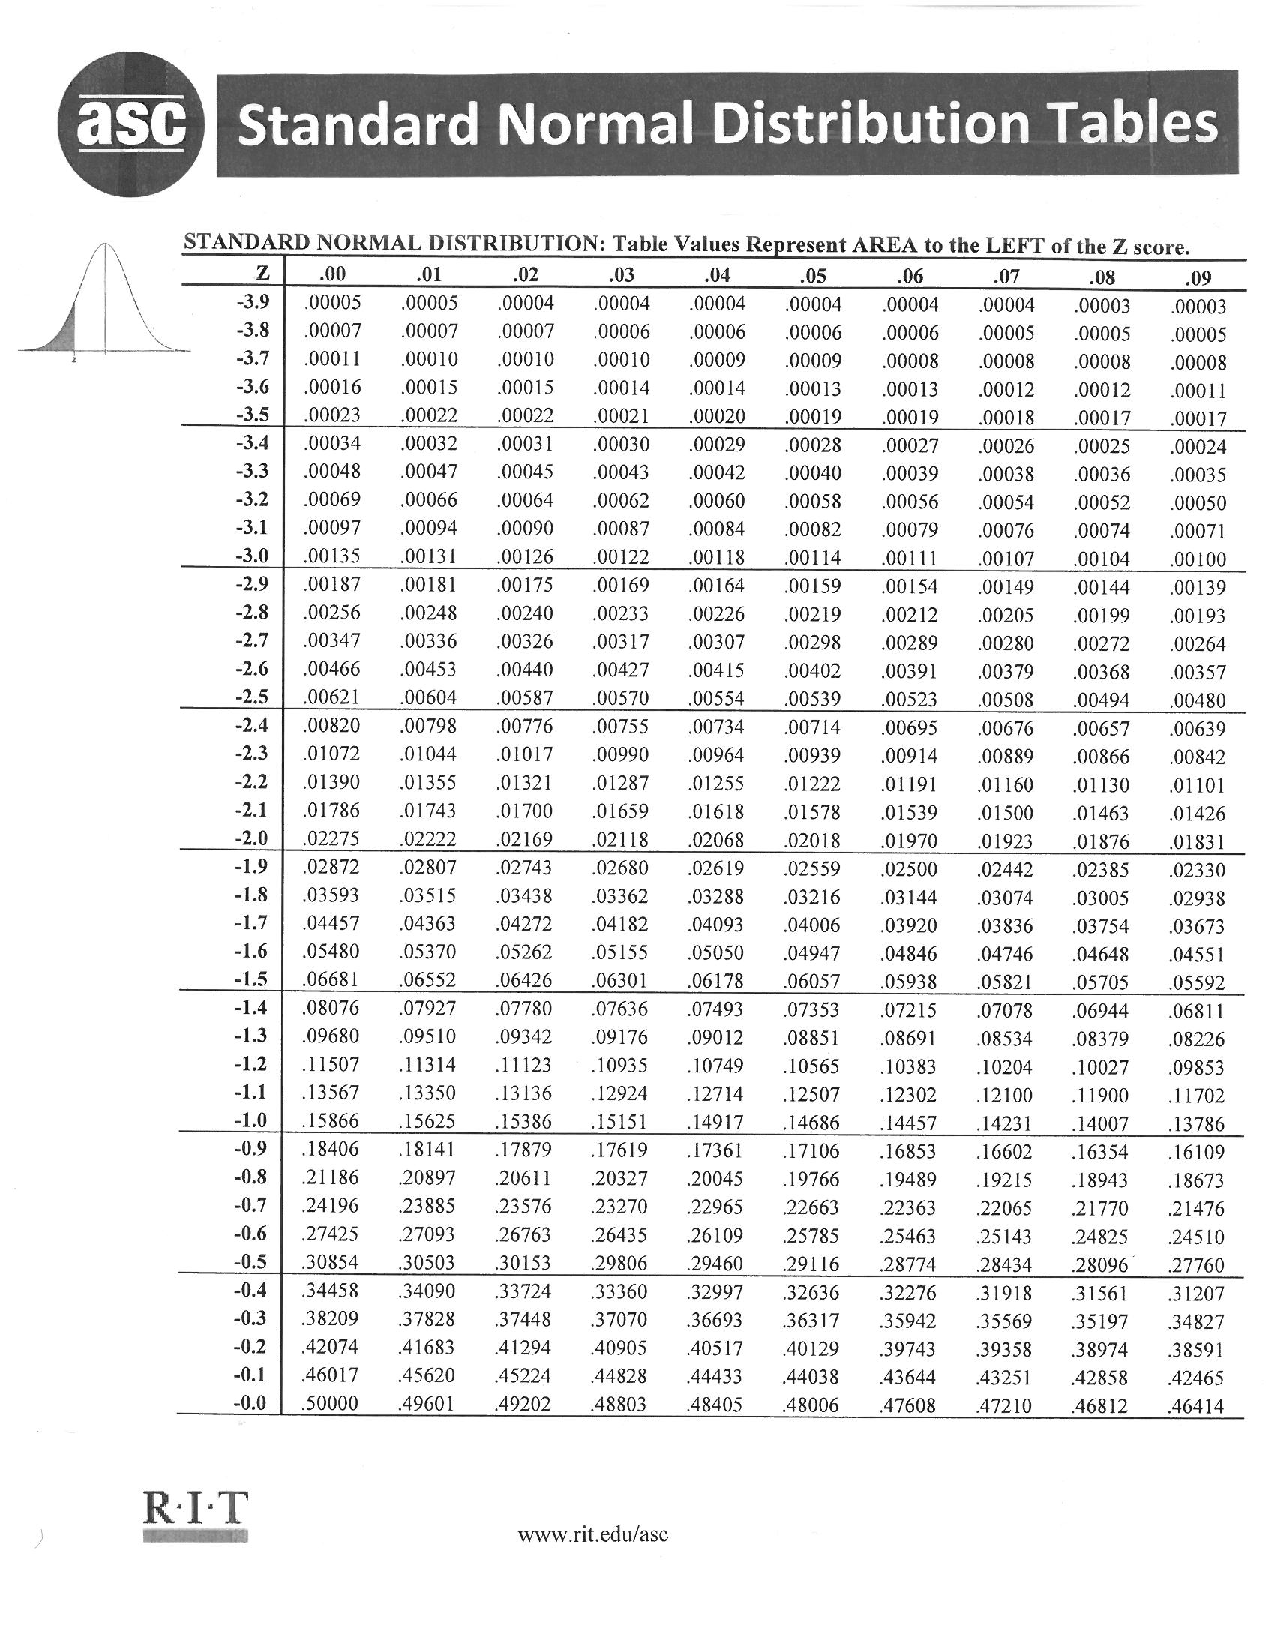
\includepdf[pages={1,2}]{NormalTable}

\newpage

\section{Rules for Derivatives}
\begin{multicols}{2}
\begin{itemize}
  \item $\displaystyle\frac{d}{dx} (c) = 0$.
  \item $\displaystyle\frac{d}{dx} (x) = 1$.
  \item $\displaystyle\frac{d}{dx} (x^n) = n x^{n - 1}$.
  \item $\displaystyle\frac{d}{dx} (e^x ) = e^x$.
  \item $\displaystyle\frac{d}{dx} (\ln (x)) = \frac{1}{x}$.
  \item $\displaystyle\frac{d}{dx} (a^x) = a^x \ln (a)$. 
  \item $\displaystyle\frac{d}{dx} (\sin x) = \cos x$. 
  \item $\displaystyle\frac{d}{dx} (\cos x) = -\sin x$.
  \item $\displaystyle\frac{d}{dx} (\tan x) = \sec^2 (x)$.
  \item $\displaystyle\frac{d}{dx} (\cot x) = -\csc^2 (x)$.
  \item $\displaystyle\frac{d}{dx} (\sec x ) = \sec x \tan x$.
  \item $\displaystyle\frac{d}{dx} (\csc x) = -\csc x \cot x$.
\end{itemize}
\end{multicols}

\section{Rules for Integrals}
\begin{multicols}{2}
\begin{itemize}
\item $\displaystyle\int 0 \, dx = C$.
\item $\displaystyle\int 1 \, dx = x + C$.
\item $\displaystyle\int x^n \, dx = \frac{x^{n + 1}}{n + 1} + C$.
\item $\displaystyle\int e^x \, dx = e^x + C$.
\item $\displaystyle\int \frac{1}{x} \, dx = \ln (x) + C$.
\item $\displaystyle\int a^x \, dx = \frac{a^x}{\ln a} + C$.
\item $\displaystyle\int \cos x \, dx = \sin x + C$. 
\item $\displaystyle\int \sin x \, dx = -\cos x + C$.
\item $\displaystyle\int \sec^2 (x) \, dx = \tan x + C$.
\item $\displaystyle\int \csc^2 (x) \, dx = - \cot x + C$.
\item $\displaystyle\int \tan x \sec x \, dx = \sec x + C$.
\item $\displaystyle\int \cot x \csc x \, dx = -\csc x + C$.
\end{itemize}
\end{multicols}

\section{General Rules}

\begin{itemize}
\item $\displaystyle\frac{d}{dx} (f (x) g(x)) = f' (x) g(x) + f(x) g' (x)$.
\item $\displaystyle \frac{d}{dx} \Big( \frac{f(x)}{g(x)} \Big) = \frac{f' (x) g(x) - f(x) g'(x)}{(g(x))^2}$.
\item $\displaystyle \frac{d}{dx} \big( f (g(x)) \big) = f' (g(x)) g' (x)$.
\end{itemize}

\end{document}

